\documentclass{article}

\usepackage{listings}
\usepackage{color}
%https://stackoverflow.com/questions/3175105/inserting-code-in-this-latex-document-with-indentation
\definecolor{dkgreen}{rgb}{0,0.6,0}
\definecolor{gray}{rgb}{0.5,0.5,0.5}
\definecolor{mauve}{rgb}{0.58,0,0.82}

\lstset{frame=tb,
  language=Java,
  aboveskip=3mm,
  belowskip=3mm,
  showstringspaces=false,
  columns=flexible,
  basicstyle={\small\ttfamily},
  numbers=none,
  numberstyle=\tiny\color{gray},
  keywordstyle=\color{blue},
  commentstyle=\color{dkgreen},
  stringstyle=\color{mauve},
  breaklines=true,
  breakatwhitespace=true,
  tabsize=3
}
%https://stackoverflow.com/questions/3175105/inserting-code-in-this-latex-document-with-indentation
\usepackage[utf8]{inputenc}
\usepackage{graphicx}

\usepackage[legalpaper, margin=.5in]{geometry}
\title{Testing Plan}
\author{Josh Carroll & James Driver}
\date{March 7th, 2023}
\begin{document}
\begin{titlepage}
   \begin{center}
       \vspace*{1cm}

       \textbf{Test Plan}

       \vspace{0.5cm}
        Zerg Mining Expedition
            
       \vspace{1.5cm}

       \textbf{Josh Carroll, James Viner \& Raymone Miller}

       \vfill
            
       \vspace{0.8cm}
            
       Tool Developer Qualification Course\\
       UMBC\\
       March 7th, 2023
            
   \end{center}
\end{titlepage}
\noindent\Huge\textbf{Test Plan, Mining}\\
\\
\Large{The program is designed to be an API which will help a developer in coding
an actual program. This API will consist of Zerg overlords and Zerg Drones.
The overlords will send drones out upon mining expeditions to collect and
bring back minerals that the Zerg race need to survive. As these drones are
deployed and explore the map they will suggest a route that is the best path
to the minerals according to the drone’s current knowledge of the map.}\\
\\

\\
\noindent\Large\textbf{Instructor provided Files}
\begin{itemize}
  \item \textbf{~/timeout.py}\\
  {Defines functions needed for a program timeout.}
   \item \textbf{~/map.py}\\
  {defines location, map, mineral context, and drone context classes.}
   \item \textbf{~/begin\_mining\_expedition.py}\\
  {attempts to run a mining expedition w/ data types needed.}
   \item \textbf{~/sample\_classes.py}\\
  {defines dashboard, Drone and Overlord classes.}
     \item \textbf{~/maps}\\
  {contains test maps.}
\end{itemize}

\noindent\Large\textbf{Sample Files}
\begin{itemize}
  \item \textbf{None yet listed}\\
\end{itemize}

\Large\textbf{TC1:Installation}
\begin{enumerate}
    \item \textit{git clone git@git.umbc.tc:tdqc/tdqc12/carroll/mining.git}
    \item \textit{cd mining}\\
    \textbf{Expected:}{mining directory is created}\\
\end{enumerate}
\large{prerequisites: In mining directory}\\
\Large\textbf{TC2:Correct Branch}
\begin{enumerate}
    \item \textit{git branch}\\
    \textbf{Expected:}{main is default branch}
\end{enumerate}
\noindent\huge\textbf{Common Test Cases}\\
\newpage
\Large\textbf{TC3: Initialize a Dashboard}\\
\indent\large{prerequisites: User's code must initialize a dashboard.}\\
\begin{lstlisting}
#!/usr/bin/env python3
"""Test main."""
from tkinter import Tk, mainloop

from mining.GUI.dashboard import Dashboard

root = Tk()

example = Dashboard(root)

mainloop()
\end{lstlisting}
\begin{description}
    \textbf{Expected:}{The program will initialize a GUI dashboard that will be present to the user.}
    \begin{figure}[htp]
    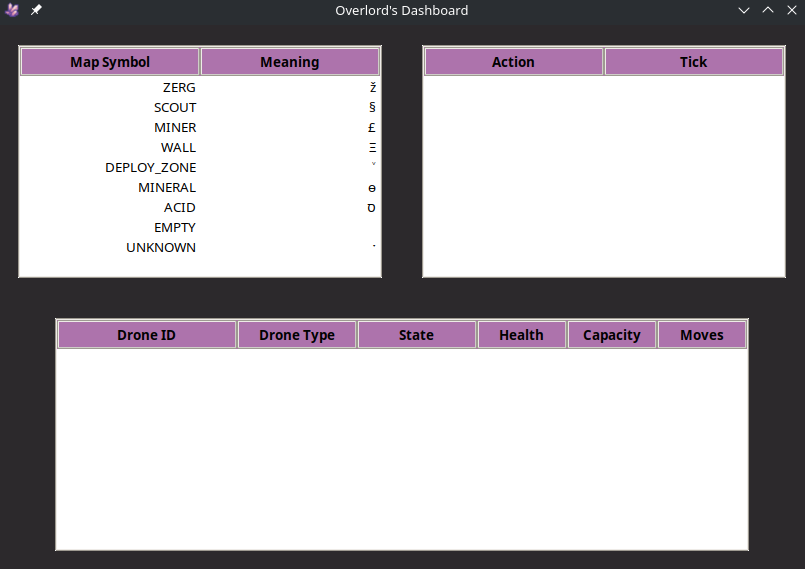
\includegraphics[width=10cm, height=7cm]{testcase3.png}
    
    \caption{T3 Output}
    \label{fig:galaxy}
\end{figure}
\end{description}
\newpage
\Large\textbf{TC4: Add a map}\\
\indent\large{prerequisites: User's code must have previously initialized a dashboard.}\\
\begin{lstlisting}
#!/usr/bin/env python3
"""Test main."""
from tkinter import Tk, mainloop
from mining.GUI.dashboard import Dashboard
from mining.zerg_units.zerg import Zerg
from mining.zerg_units.overlord import Overlord
from mining.utils.icon import Icon
from mining.utils.map import Map
from mining.GUI.dashboard import Dashboard
root = Tk()
example = Dashboard(root)
cocopebbles = Map(0.0)
example.create_map_gui(cocopebbles)
mainloop()

\end{lstlisting}
\begin{description}
    \textbf{Expected:}{The program will initialize a GUI dashboard that will be present to the user as well as one map that will be filled with unknown tiles.}
    \begin{figure}[htp]
    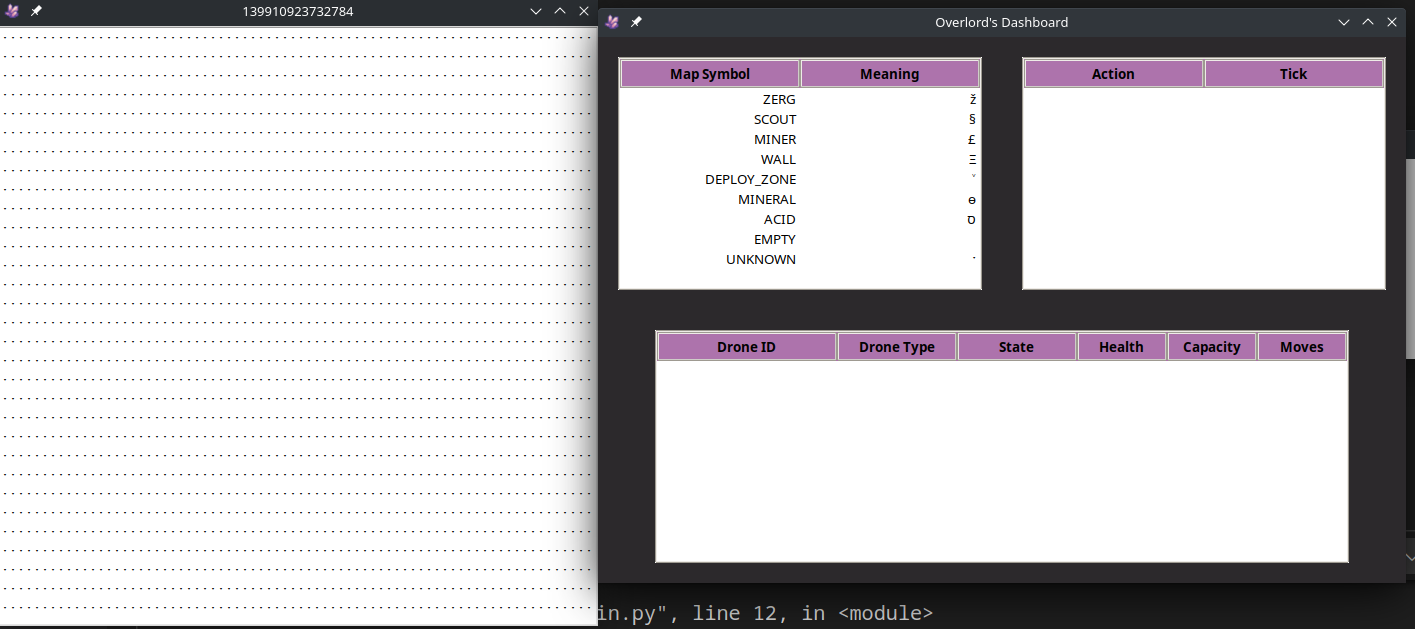
\includegraphics[width=15cm, height=7cm]{testcase4.png}
    
    \caption{T4 Output}
    \label{fig:galaxy}
\end{figure}
\end{description}

\newpage
\Large\textbf{TC5: Add a drone to the dashboard}\\
\indent\large{prerequisites: User's code must have previously initialized a dashboard.}\\
\begin{lstlisting}
#!/usr/bin/env python3
"""Test main."""
from tkinter import Tk, mainloop
from mining.GUI.dashboard import Dashboard
from mining.zerg_units.drones.scout import ScoutDrone
from mining.zerg_units.zerg import Zerg
from mining.zerg_units.overlord import Overlord
from mining.utils.icon import Icon
root = Tk()

example = Dashboard(root)

new_overlord = Overlord(5, 10, example)

new_drone = ScoutDrone(new_overlord)
example.add_drone_to_tree(new_drone)

mainloop()
\end{lstlisting}
\begin{description}
    \textbf{Expected:}{The program will initialize a GUI dashboard that will be present to the user, and will fill the drone table with at least one drone}
    \begin{figure}[htp]
    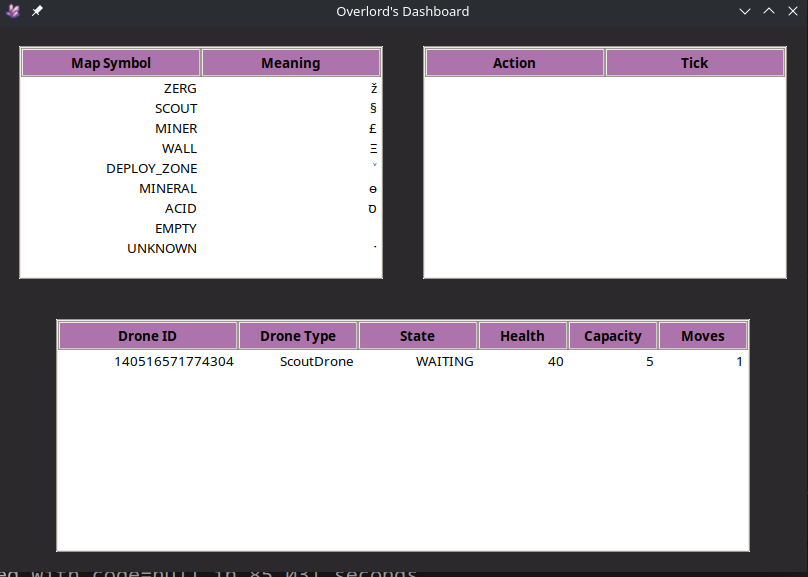
\includegraphics[width=15cm, height=7cm]{testcase5.png}
    
    \caption{T5 Output}
    \label{fig:galaxy}
\end{figure}
\end{description}


\newpage
\Large\textbf{TC6: Add a action to the action table}\\
\indent\large{prerequisites: User's code must have previously initialized a dashboard.}\\
\begin{lstlisting}
#!/usr/bin/env python3
"""Test main."""
from tkinter import Tk, mainloop
from mining.GUI.dashboard import Dashboard
from mining.zerg_units.drones.scout import ScoutDrone
from mining.zerg_units.zerg import Zerg
from mining.zerg_units.overlord import Overlord
from mining.utils.icon import Icon
root = Tk()

example = Dashboard(root)

example.insert_action("Action", "Tick")
            
mainloop()  

\end{lstlisting}
\begin{description}
    \textbf{Expected:}{The program will initialize a GUI dashboard that will be present to the user, and will fill the action table with at least one action and tick.}
    \begin{figure}[htp]
    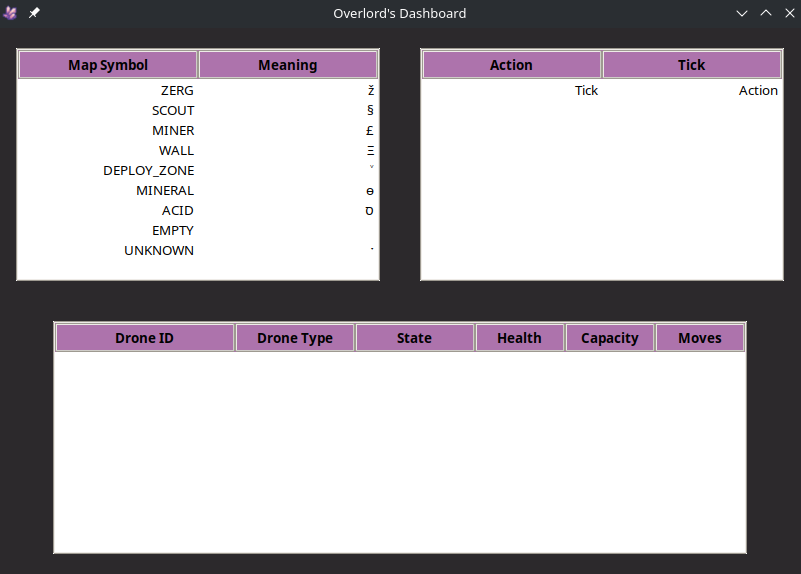
\includegraphics[width=15cm, height=7cm]{testcase6.png}
    
    \caption{T6 Output}
    \label{fig:galaxy}
\end{figure}
\end{description}


\newpage
\Large\textbf{TC7: Reading a map into the GUI}\\
\indent\large{prerequisites: User's code must have previously initialized a dashboard. The user must also have a map object already made. We accomplished this by using a function to 
read a file into a map}\\
\begin{lstlisting}
#!/usr/bin/env python3
"""Test main."""
from tkinter import Tk, mainloop

from mining.GUI.dashboard import Dashboard
from mining.utils.map import Map
from mining.utils.tile import Tile
from mining.zerg_units.drones.scout import ScoutDrone
from mining.zerg_units.zerg import Zerg
from mining.zerg_units.overlord import Overlord
from mining.utils.coordinate import Coordinate
from mining.utils.icon import Icon



def file_read(file_name):
    """
    Reads a file into a map. This function is just used
    for testing purposes and will not be apart of the main product.
    Argument:
        file_name (string): Name of the file that will be read.
    """
    new_map = Map(0.0)
    Tile_dict = {}
    fp = open(file_name, "r")
    linecounter = 1
    for line in fp:
        lettercounter = 0 
        for letter in line:
            if letter == '\n':
                letter = ' '
            elif letter.isnumeric():
                letter = '*'
            Coordinate = (lettercounter, linecounter)
            tile = Tile(Coordinate, Icon(letter))
            Tile_dict[Coordinate] = tile
            lettercounter += 1
        linecounter += 1
    new_map._stored_tiles_ = Tile_dict
    return new_map

root = Tk()
new_map = file_read("maps/map04.txt")

example = Dashboard(root)

example.create_map_gui(new_map)
example.update_maps([])

mainloop()

\end{lstlisting}
\begin{description}
    \textbf{Expected:}{The program will initialize a GUI dashboard that will be present to the user, and will fill the map window with the map that was read.}
    \begin{figure}[htp]
    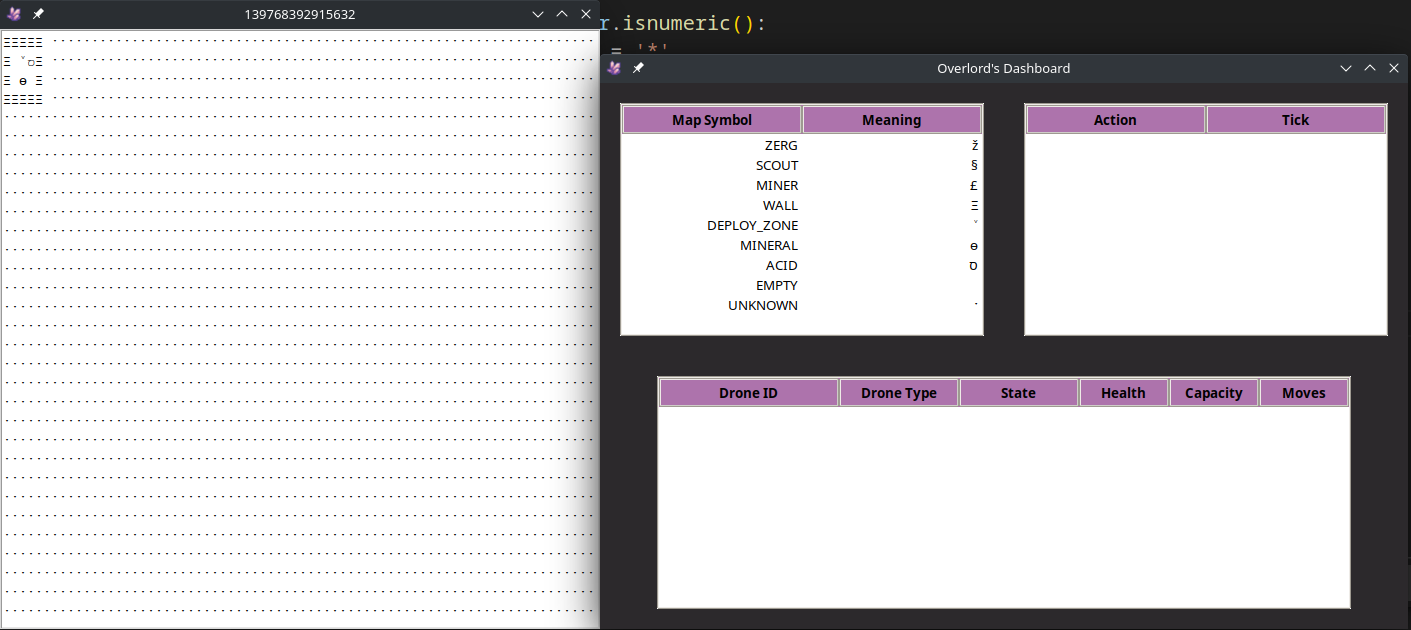
\includegraphics[width=15cm, height=7cm]{testcase7.png}
    
    \caption{T7 Output}
    \label{fig:galaxy}
\end{figure}
\end{description}


\newpage
\Large\textbf{TC8: Reading  multiple maps into the GUI}\\
\indent\large{prerequisites: User's code must have previously initialized a dashboard. The user must also have map objects already made. We accomplished this by using a function to 
read a file into a map}\\
\begin{lstlisting}
#!/usr/bin/env python3
"""Test main."""
from tkinter import Tk, mainloop

from mining.GUI.dashboard import Dashboard
from mining.utils.map import Map
from mining.utils.tile import Tile
from mining.zerg_units.drones.scout import ScoutDrone
from mining.zerg_units.zerg import Zerg
from mining.zerg_units.overlord import Overlord
from mining.utils.coordinate import Coordinate
from mining.utils.icon import Icon



def file_read(file_name):
    """
    Reads a file into a map. This function is just used
    for testing purposes and will not be apart of the main product.
    Argument:
        file_name (string): Name of the file that will be read.
    """
    new_map = Map(0.0)
    Tile_dict = {}
    fp = open(file_name, "r")
    linecounter = 1
    for line in fp:
        lettercounter = 0 
        for letter in line:
            if letter == '\n':
                letter = ' '
            elif letter.isnumeric():
                letter = '*'
            Coordinate = (lettercounter, linecounter)
            tile = Tile(Coordinate, Icon(letter))
            Tile_dict[Coordinate] = tile
            lettercounter += 1
        linecounter += 1
    new_map._stored_tiles_ = Tile_dict
    return new_map

root = Tk()
new_map = file_read("maps/map04.txt")
new_map2 = file_read("maps/map03.txt")

example = Dashboard(root)

example.create_map_gui(new_map)
example.create_map_gui(new_map2)
example.update_maps([])

mainloop()

\end{lstlisting}
\begin{description}
    \textbf{Expected:}{The program will initialize a GUI dashboard that will be present to the user, and will fill both map windows with the maps that were read.}
    \begin{figure}[htp]
    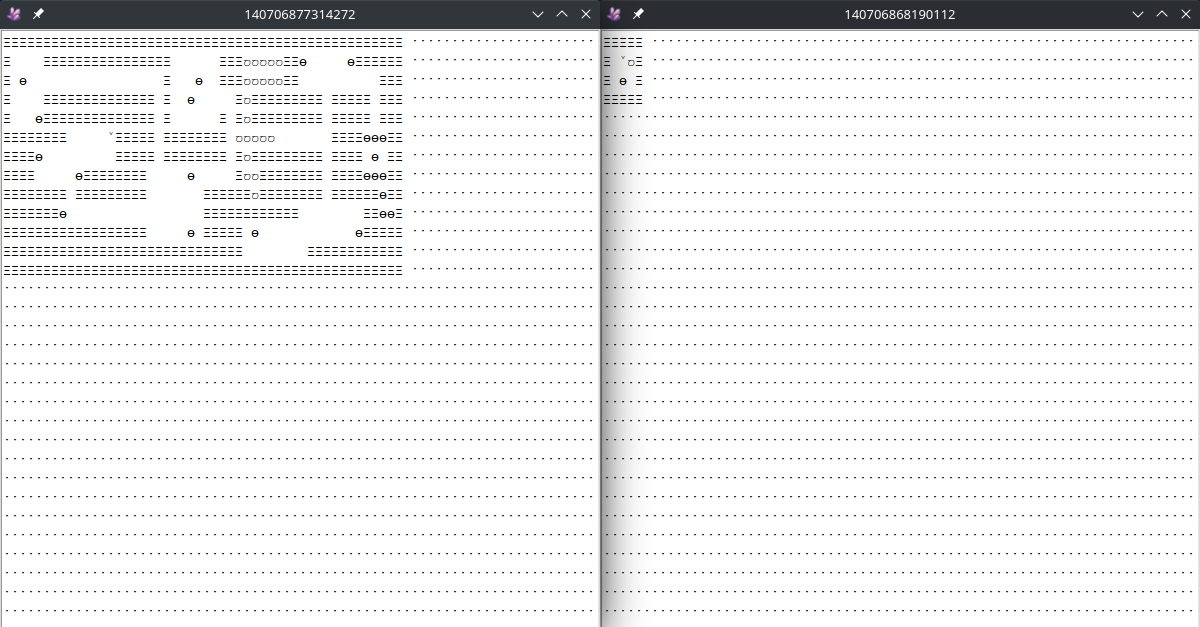
\includegraphics[width=15cm, height=7cm]{testcase8-1.png}
    
    \caption{T8 Output}
    \label{fig:galaxy}
\end{figure}
    \begin{figure}[htp]
    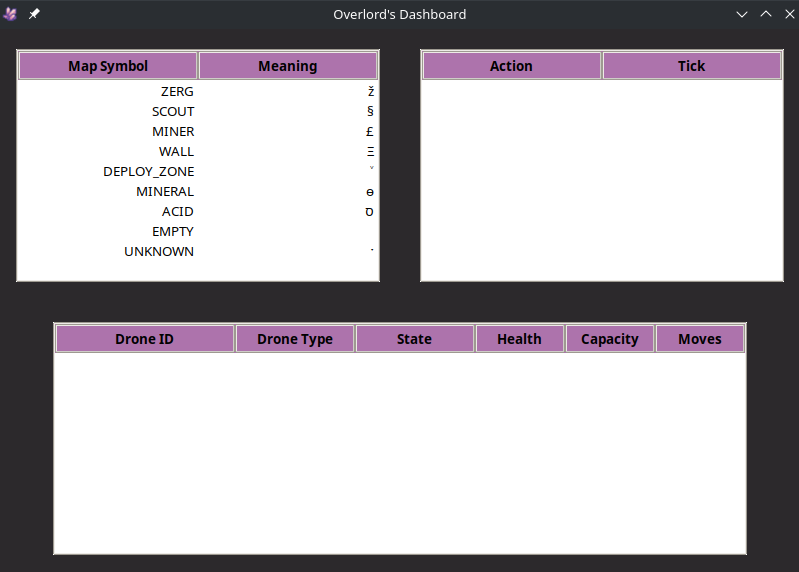
\includegraphics[width=15cm, height=7cm]{testcase8-2.png}
    
    \caption{T8 Output}
    \label{fig:galaxy}
\end{figure}
\end{description}


\newpage
\Large\textbf{TC9: Reading four maps into the GUI}\\
\indent\large{prerequisites: User's code must have previously initialized a dashboard. The user must also have map objects already made. We accomplished this by using a function to 
read a file into a map}\\
\begin{lstlisting}
#!/usr/bin/env python3
"""Test main."""
from tkinter import Tk, mainloop

from mining.GUI.dashboard import Dashboard
from mining.utils.map import Map
from mining.utils.tile import Tile
from mining.zerg_units.drones.scout import ScoutDrone
from mining.zerg_units.zerg import Zerg
from mining.zerg_units.overlord import Overlord
from mining.utils.coordinate import Coordinate
from mining.utils.icon import Icon



def file_read(file_name):
    """
    Reads a file into a map. This function is just used
    for testing purposes and will not be apart of the main product.
    Argument:
        file_name (string): Name of the file that will be read.
    """
    new_map = Map(0.0)
    Tile_dict = {}
    fp = open(file_name, "r")
    linecounter = 1
    for line in fp:
        lettercounter = 0 
        for letter in line:
            if letter == '\n':
                letter = ' '
            elif letter.isnumeric():
                letter = '*'
            Coordinate = (lettercounter, linecounter)
            tile = Tile(Coordinate, Icon(letter))
            Tile_dict[Coordinate] = tile
            lettercounter += 1
        linecounter += 1
    new_map._stored_tiles_ = Tile_dict
    return new_map

root = Tk()
new_map = file_read("maps/map04.txt")
new_map2 = file_read("maps/map03.txt")
new_map3 = file_read("maps/map02.txt")
new_map4 = file_read("maps/map01.txt")
example = Dashboard(root)

example.create_map_gui(new_map)
example.create_map_gui(new_map2)
example.create_map_gui(new_map3)
example.create_map_gui(new_map4)
example.update_maps([])

mainloop()
\end{lstlisting}
\begin{description}
    \textbf{Expected:}{The program will initialize a GUI dashboard that will be present to the user, and will fill both map windows with the maps that were read.}
    \begin{figure}[htp]
    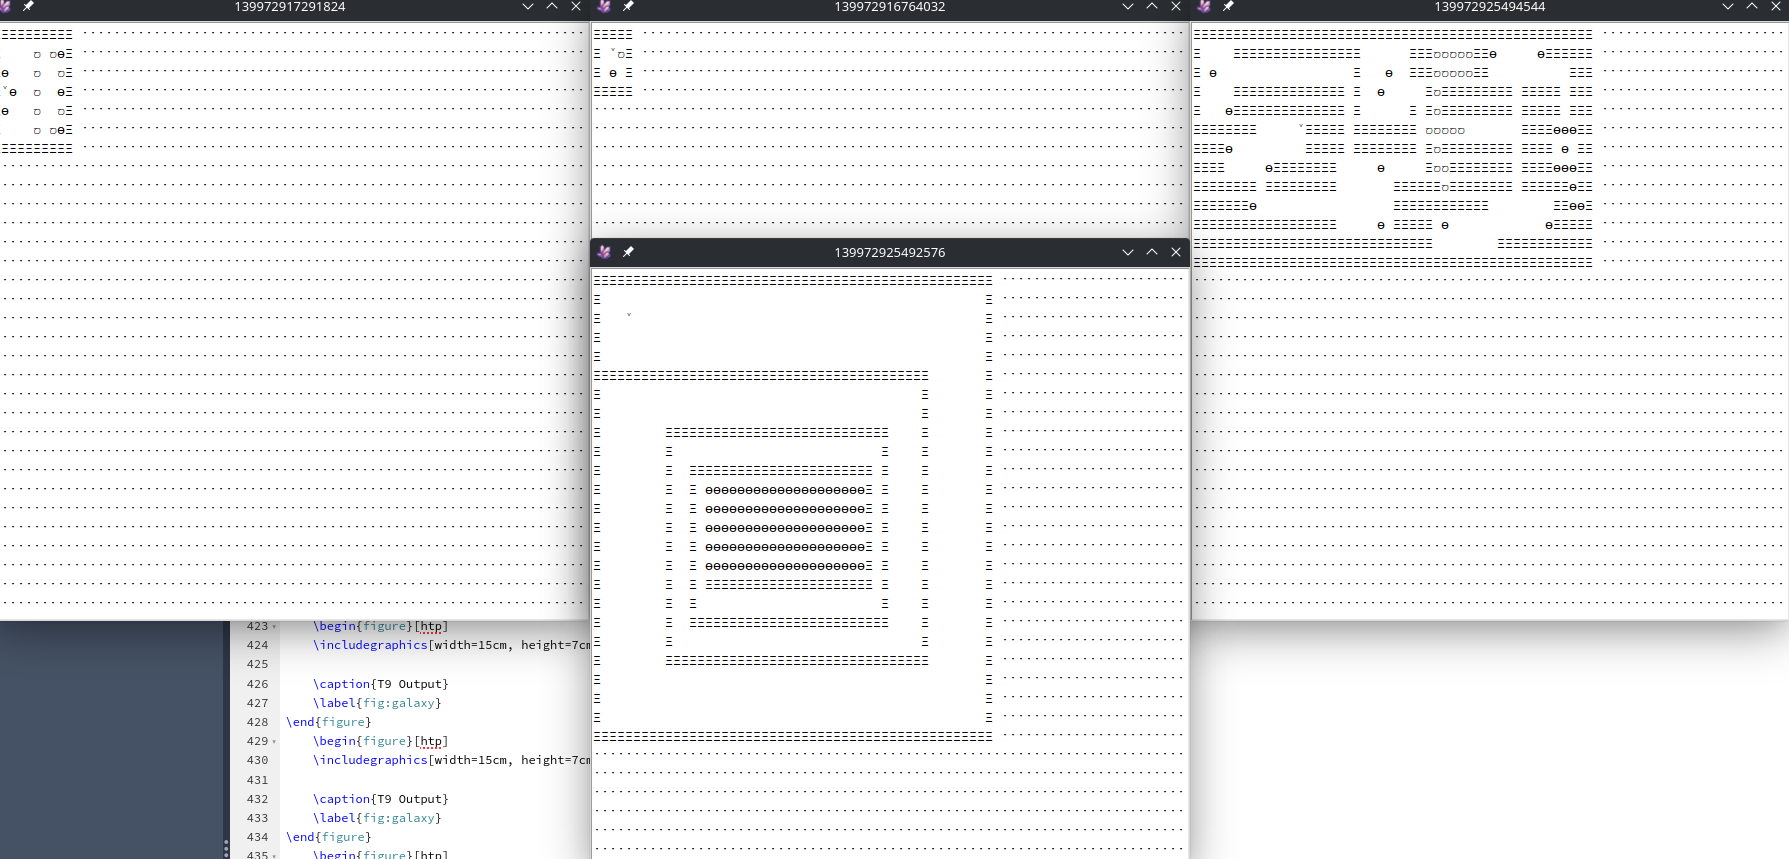
\includegraphics[width=15cm, height=7cm]{testcase9.png}
    
    \caption{T9 Output}
    \label{fig:galaxy}
\end{figure}
    \begin{figure}[htp]
    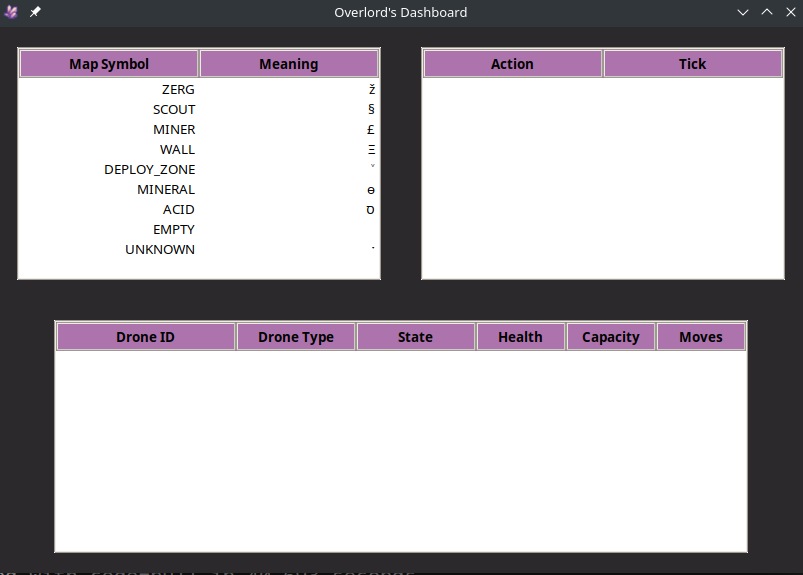
\includegraphics[width=15cm, height=7cm]{testcase9-1.png}
    
    \caption{T9 Output}
    \label{fig:galaxy}
\end{figure}




\newpage
\Large\textbf{TC10: Launching mining expedition without data.}\\
\indent\large{prerequisites: User must be in mining directory with the begin\_mining\_expedition.py. Type in the command "python3 begin\_mining\_expedition.py" into the terminal.\\
\begin{enumerate}
    \item \textit{Put the following options in testing menu}
    \item \textit{set "Ticks" equal to 100}\\
    \item \textit{set "Refined Minerals" equal to 100}\\
    \item \textit{set "Refresh Delay" equal to 0.1}\\
    \item \textit{Click the start button}\\
    \textbf{Expected:}{The user will get an Error about the program getting no data.}\\
\end{enumerate}

\end{document}

